% !TEX root = ../ba_scrreprt_master.tex
% @author Marcel Ruland (2018)

\newcommand{\hnaught}{\textit{H}\textsubscript{\addfontfeature{Numbers=Lining}0}}
\newcommand{\hone}{\textit{H}\textsubscript{\addfontfeature{Numbers=Lining}1}}


\chapter{\significance}
\label{ch:significance}
\chapterintro{Significance tests are one of the most widely used statistical tools in academic work of virtually all disciplines dealing with some sort of numerical data. As is the case with most widely used tools, the temptation to merely learn its application and neglect conceptual understanding is present. I will try and bypass this fallacy by devoting section \ref{sec:signat} to the concept of statistical significance. The following section \ref{sec:sigmet} describes the creation of a null hypothesis to establish a baseline against which to test for significance. Finally, section \ref{sec:sigres} discusses the results.}

\section{The Nature of Significance}
\label{sec:significancenature}
In a classic experimental setting, one distinguishes between a control group and an experimental group. In the control group, all variables are held constant, whereas in the experimental group a single variable is modified in some way. Naturally, the object of interest are the potential effects the changes to the variable might have on the experimental group. Speaking more abstractly, experimental and control group are two populations with some population parameter \(p\). Let us assume that its value \(p_e\) in the experimental group is different from its value \(p_c\) in the control group. The aim of significance tests is to objectively state whether the difference


\begin{quote}\small\singlespacing
``We are inclined to think that as far as a particular hypothesis is concerned, no test based upon the theory of probability can by itself provide any valuable evidence of the truth or falsehood of that hypothesis. But we may look at the purpose of test from another view-point. Without hoping to know whether each separate hypothesis is true or false, we may search for rules to govern our behavior with regard to them, in following which we insure that, in the long run of experience, we shall not be too often wrong.''

~ \hfill \citep[\pnum{TBA}]{neyman33}
\end{quote}

\paragraph{Numerical vs applied significance} A certain kind of lens might have a positive effect on sight that is statistically significant. At the same time, this positive effect can be so small that humans are unable to perceive a difference. While this effect is undoubtedly significant numerically, no one would pay money for a lens whose effect they do not perceive. In that sense, significance alone must not be accepted blindly, because significance in turn is blind to effect size or scale \citep[\cnum{8}]{frost17}.

\section{Method}
\label{sec:significancemethod}
The crucial missing piece for establishing the significance of a rule is a base case\dash or base distribution, so to speak\dash against which to compare the rule's probability. In other words: while there obviously is a real distribution, we lack a null distribution for comparison. The methodological approach I take, therefore, is to create a null distribution, which then serves as a basis for the real rules' probabilities to be tested for significance. This is in some respects similar to\dash and certainly inspired by\dash \citet[\pnum{10~f.}]{abuzhaya17}.

We take one of the ten sequences in the corpus. For each of the 11 dimensions individually (cf.~table \ref{tab:events}), we shuffle the events with respect to their start points in time, but leave their duration untouched, i.e.~we leave the position of their time end points untouched \emph{with respect to their time start points.} We also do not add or remove any events. This process is done for all 11 dimensions. Figure \ref{fig:null} gives an example hereof. The top half of the figure is an excerpt of real data taken from a sequence in the corpus. We see three events of type \code{mother\_voc}, three shorter events of type \code{mother\_gaze\_infant}, one longer event of type \code{infant\_gaze\_mother}, etc.\footnote{The excerpt taken did not contain events of all 11 types, empty dimensions have simply been omitted in the graphic.} The bottom half of the figure shows a corresponding null distribution. Notice how \code{mother\_voc} still contains the same three events of the same length but in a different temporal order. The same is true for all other dimensions.

We now have a distribution of the sequence which contains the exact same events as the real distribution, but shuffled in their temporal order. In other words, the only thing that has changed is the temporal arrangement of the events \emph{with respect to one another.} We will call this a null \textbf{sequence} and create 100 of its kind.\footnote{Having chosen to create exactly 100 null sequences for every real sequence has\dash admittedly\dash little motivation. Were it not for us being used to count in base 10, the chosen number\dash let it be \textit{k}\dash would in all probability have been different. However, this is not a big issue. The higher the number of created null sequences is, the smaller the margin of error for the p-values will be. That is to say, \textit{k} being too small poses issues, but \textit{k} being too large does not. With the chosen value of \textit{k}~=~100, the margin of error is SOME VALUE, which is GREAT BECAUSE WHAT?}
We go through the same process for all of the 10 sequences and end up having 1000 null distributions, with 100 each corresponding to a given sequence.

Finally, to evaluate a rule's significance we take the distribution of its probability in all of the 1000 null distributions, i.e.~we obtain a probability distribution with 1000 data points. We then test for significance at \(\alpha\)~=~0.05 using some test or another. % Is this distribution normal? Central limit theorem?

\begin{figure}
	\centering
	% !TEX root = ../../scrreprt_figures/ba_scrreprt_figures.tex
% @author Marcel Ruland (2018)

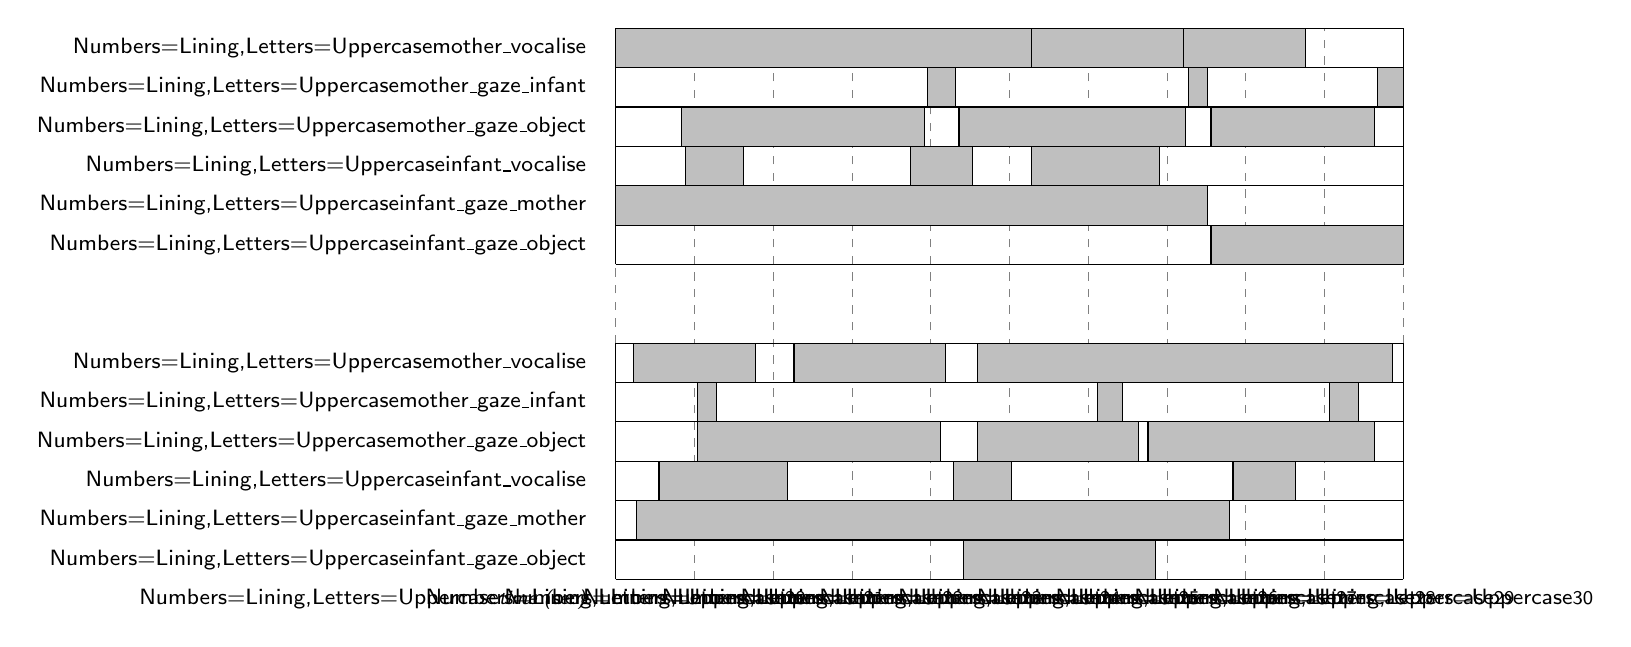
\begin{tikzpicture}[
	node distance=0 and 0,  % y, x for fuck knows what reason
	every node/.append style={font=\footnotesize\sffamily\addfontfeature{Numbers=Lining,Letters=Uppercase}}]
%	\draw [help lines, dashed] (0,0) grid (13,7);
	
	% time line
	% annotations
	\node [anchor=east] at (2.75, -0.25) {\textit{\scriptsize{time (sec)}}};
	\foreach \i in {20, 21,..., 29, 30}
		\node at ({\i-17},-0.25) {\scriptsize{\i}};
	% small vertical help lines
	\draw [help lines, dashed] (3,3) -- (3,4);
	\draw [help lines, dashed] (13,3) -- (13,4);
	% long vertical help lines
	\foreach \i in {4, 5,..., 11, 12}
		\draw [help lines, dashed] (\i,0) -- (\i,7);
	
	%% grids
	% vertical lines
	\foreach \i in {3, 13}{
		\draw (\i,4) -- (\i,7);  % top
		\draw (\i,0) -- (\i,3);  % bottom
	}
	% horizontal lines
	\foreach \i in {0, 0.5,..., 2.5, 3, 4, 4.5,..., 6.5, 7}  % top and bottom
		\draw (3,\i) -- (13,\i);
%	% annotations, not happy with them the way they are
%	\node[rotate=-90, anchor=south] at (13,5.5) {\textsc{real}};
%	\node[rotate=-90, anchor=south] at (13,1.5) {\textsc{null}};
		
	%% labels
	\foreach \i in {0.25, 4.25}{  % top and bottom
		\node[anchor=east] at (2.75,{\i+2.5}) {\code{mother\_vocalise}};
		\node[anchor=east] at (2.75,{\i+2}) {\code{mother\_gaze\_infant}};
		\node[anchor=east] at (2.75,{\i+1.5}) {\code{mother\_gaze\_object}};
		\node[anchor=east] at (2.75,{\i+1}) {\code{infant\_vocalise}};
		\node[anchor=east] at (2.75,{\i+0.5}) {\code{infant\_gaze\_mother}};
		\node[anchor=east] at (2.75,\i) {\code{infant\_gaze\_object}};
	}
	
	%% annotations
	% top
	\draw [fill=lightgray] (3,6.5) rectangle (8.279,7);
	\draw [fill=lightgray] (8.279,6.5) rectangle (10.206,7);
	\draw [fill=lightgray] (10.206,6.5) rectangle (11.76,7);

	\draw [fill=lightgray] (6.96,6) rectangle (7.32,6.5);
	\draw [fill=lightgray] (10.28,6) rectangle (10.52,6.5);
	\draw [fill=lightgray] (12.68,6) rectangle (13,6.5);
	
	\draw [fill=lightgray] (3.84,5.5) rectangle (6.92,6);
	\draw [fill=lightgray] (7.36,5.5) rectangle (10.24,6);
	\draw [fill=lightgray] (10.56,5.5) rectangle (12.64,6);
	
	\draw [fill=lightgray] (3.887,5) rectangle (4.624,5.5);
	\draw [fill=lightgray] (6.74,5) rectangle (7.53,5.5);
	\draw [fill=lightgray] (8.279,5) rectangle (9.909,5.5);
	
	\draw [fill=lightgray] (3,4.5) rectangle (10.52,5);

	\draw [fill=lightgray] (10.56,4) rectangle (13,4.5);
	% bottom
	\draw [fill=lightgray] (7.592,2.5) rectangle (12.871,3);
	\draw [fill=lightgray] (5.264,2.5) rectangle (7.191,3);
	\draw [fill=lightgray] (3.221,2.5) rectangle (4.775,3);

	\draw [fill=lightgray] (12.069,2) rectangle (12.429,2.5);
	\draw [fill=lightgray] (4.039,2) rectangle (4.279,2.5);
	\draw [fill=lightgray] (9.115,2) rectangle (9.435,2.5);
	
	\draw [fill=lightgray] (4.04,1.5) rectangle (7.12,2);
	\draw [fill=lightgray] (9.76,1.5) rectangle (12.64,2);
	\draw [fill=lightgray] (7.59,1.5) rectangle (9.64,2);
	
	\draw [fill=lightgray] (7.287,1) rectangle (8.024,1.5);
	\draw [fill=lightgray] (10.84,1) rectangle (11.63,1.5);
	\draw [fill=lightgray] (3.55,1) rectangle (5.18,1.5);
	
	\draw [fill=lightgray] (3.27,0.5) rectangle (10.79,1);

	\draw [fill=lightgray] (7.42,0) rectangle (9.86,0.5);
\end{tikzpicture}
	\caption{An excerpt of a real sequence (top) and a corresponding null distribution (bottom). Note how events are shuffled with respect to their position in time, whereas their duration and number has been left untouched.}
	\label{fig:null}
\end{figure}
\begin{figure}[h]
	\centering
	% !TEX root = ../../scrreprt/ba_scrreprt_master.tex
% @author Marcel Ruland (2018)

% semantic commands
\newcommand{\nullnode}{100 Null}
\newcommand{\samplenode}{sample}
\newcommand{\commentfont}[1]{{\rmfamily\tiny\textit{#1}}}
\newcommand{\annotationcounter}[1]{{\rmfamily\addfontfeature{Numbers=Lining}\scriptsize\textbf{#1.~}}}

% coordinates
\newcommand{\nully}{8}			% y-position of null nodes
\newcommand{\sampley}{5}		% y-position of sample nodes
\newcommand{\realx}{6}			% x position of leftmost real node
\newcommand{\realy}{\sampley}	% y-position of real nodes

% incrementers
\newcommand{\nullinc}{1.5}			% increment for null nodes
\newcommand{\sampleinc}{2}		% increment for sample nodes
\newcommand{\realinc}{1}			% increment for real nodes
\newcommand{\realtonullinc}{0.3}	% increment for real to null arrows

% other
\newcommand{\nodeoffset}{0.5}			% offset for \cdots
\newcommand{\annotationwidth}{1.5cm}	% width of annotations on left side
% gaussian function for plot
\pgfmathdeclarefunction{gauss}{2}{\pgfmathparse{1/(#2*sqrt(2*pi))*exp(-((x-#1)^2)/(2*#2^2))}}

\begin{tikzpicture}[
	every node/.append style={
		font=\sffamily\scriptsize\addfontfeature{
%			Numbers=Monospaced,
			Numbers=Lining,
			Letters=Uppercase
		}
	},
	node distance = 1 and 0.5,
	align=center
]
	% help lines
%	\draw[help lines, dashed] (0,0) grid (10,10);
	
	
	%%% NODES
	% null nodes
	\node[draw] at ({0 + 0*\nullinc},\nully)   (null1)  {\nullnode \\ 1};
	\node[draw] at ({0 + 1*\nullinc},\nully)   (null2)  {\nullnode \\ 2};
	\node[draw] at ({0 + 2*\nullinc},\nully)   (null3)  {\nullnode \\ 3};
	\node[draw] at ({0 + 3*\nullinc + \nodeoffset},\nully)   (null10) {\nullnode \\ 10};
	
	% sample nodes
	\node[draw] at ({0.5 + 0*\sampleinc},\sampley) (sample1) {\samplenode \\ 1};
	\node[draw] at ({0.5 + 1*\sampleinc},\sampley) (sample50) {\samplenode \\ 50};
	\node[draw] at ({0.5 + 2*\sampleinc},\sampley) (sample100) {\samplenode \\ 100};
	
	% real nodes
	\node[draw, circle, minimum size=2.5em] at ({\realx + 0*\realinc},\realy) (real1) {R1};
	\node[draw, circle, minimum size=2.5em] at ({\realx + 1*\realinc},\realy) (real2) {R2};
	\node[draw, circle, minimum size=2.5em] at ({\realx + 2*\realinc},\realy) (real3) {R3};
	\node[draw, circle, minimum size=2.5em] at ({\realx + 3*\realinc + \nodeoffset},\realy) (real10) {R10};
	
	% \cdots
	\path (null3) -- node{\(\cdots\)} (null10);
	\path (sample1) -- node{\(\cdots\)} (sample50);
	\path (sample50) -- node{\(\cdots\)} (sample100);
	\path (real3) -- node{\(\cdots\)} (real10);
	
	
	%%% ARROWS
	%% null to sample arrows
	% 1st sample
	\draw[-stealth, graphgreen] (null1.south west)  to (sample1.north);
	\draw[-stealth, graphgreen] (null2.south west)  to (sample1.north);
	\draw[-stealth, graphgreen] (null3.south west)  to (sample1.north);
	\draw[-stealth, graphgreen] (null10.south west) to (sample1.north);
	
	% 50th sample
	\draw[-stealth, graphgreen] (null1.south)  to (sample50.north);
	\draw[-stealth, graphgreen] (null2.south)  to (sample50.north);
	\draw[-stealth, graphgreen] (null3.south)  to (sample50.north);
	\draw[-stealth, graphgreen] (null10.south) to (sample50.north);
	
	% 100th sample
	\draw[-stealth, graphgreen] (null1.south east)  to (sample100.north);
	\draw[-stealth, graphgreen] (null2.south east)  to (sample100.north);
	\draw[-stealth, graphgreen] (null3.south east)  to (sample100.north);
	\draw[-stealth, graphgreen] (null10.south east) to (sample100.north);
	
	%% real to null arrows
	\draw[-stealth, graphred] (real1.north) to
					({\realx + 0*\realinc},{8.7 + 0*\realtonullinc}) to
					({0 + 0*\nullinc},{8.7 + 0*\realtonullinc}) to
					(null1.north);
					
	\draw[-stealth, graphred] (real2.north) to
					({\realx + 1*\realinc},{8.7 + 1*\realtonullinc}) to
					({0 + 1*\nullinc},{8.7 + 1*\realtonullinc}) to
					(null2.north);
					
	\draw[-stealth, graphred] (real3.north) to
					({\realx + 2*\realinc},{8.7 + 2*\realtonullinc}) to
					({0 + 2*\nullinc},{8.7 + 2*\realtonullinc}) to
					(null3.north);
					
	\draw[-stealth, graphred] (real10.north) to
					({\realx + 3*\realinc + \nodeoffset},{8.7 + 3*\realtonullinc}) to
					node[above, black]
					{\annotationcounter{1}\commentfont{generate 100 null distributions from each real sequence}}
					({0 + 3*\nullinc + \nodeoffset},{8.7 + 3*\realtonullinc}) to
					(null10.north);
	
	%% sample to plot arrows
	% nodes above plots
	\node[below=1.7cm of sample50.south] (greenplot) {};
	\node at (7.7,2.8) (redplot) {};
	
	% left plot
	\draw[-stealth, graphgreen] (sample1.south)  to (greenplot);
	\draw[-stealth, graphgreen] (sample50.south)  to (greenplot);
	\draw[-stealth, graphgreen] (sample100.south)  to (greenplot);
	
	% red plot
	\draw[-stealth, graphred] (real1.south)  to (redplot);
	\draw[-stealth, graphred] (real2.south)  to (redplot);
	\draw[-stealth, graphred] (real3.south)  to (redplot);
	\draw[-stealth, graphred] (real10.south)  to (redplot);
	
	
	
	%%% PLOTS
	%% left and green
	\begin{axis}[
		at={(110,0)},  % set origin coordinate in tikzpicture
		scale=0.5,  % half as large
		ymin=0,  % set ymin to 0
		xticklabels={,,},  % surpress digits at x-axis
		hide y axis,  % hide y axes (duh)
		axis x line*=bottom, % no box around the plot, only x and y axis
		every axis plot post/.append style={% All plots: from -2:2, 50 samples, smooth, no marks
			mark=none,
			domain=-2:2,
			samples=50,
			smooth
		}
	]
		% add normal curve
		\addplot[color=graphgreen] {gauss(0,0.5)};
		% add vertical line
		\draw[color=graphgreen, dashed] (axis cs:0,\pgfkeysvalueof{/pgfplots/ymin}) -- (axis cs:0,\pgfkeysvalueof{/pgfplots/ymax});
	\end{axis}
	
	%% right and red
	\begin{axis}[
		at={(1255,0)},  % set origin coordinate in tikzpicture
		scale=0.5,  % half as large
		ymin=0,  % set ymin to 0
		ymax=0.8,
		xticklabels={,,},  % surpress digits at x-axis
		hide y axis,  % hide y axes (duh)
		axis x line*=bottom, % no box around the plot, only x and y axis
		every axis plot post/.append style={% All plots: from -2:2, 50 samples, smooth, no marks
			mark=none,
			domain=-3:3,
			samples=50,
			smooth
		}
	]
		% add normal curve
		\addplot[color=graphred] {gauss(0,0.75)};
		% add vertical line
		\draw[color=graphred, dashed] (axis cs:0,\pgfkeysvalueof{/pgfplots/ymin}) -- (axis cs:0,\pgfkeysvalueof{/pgfplots/ymax});
	\end{axis}
	
	
	%%% THE BIG QUESTION
	\node at (5.1,0.7) (bigquestion) {\large\(\textcolor{graphgreen}{\mu_1} \stackrel{?}{=} \textcolor{graphred}{\mu_2}\)};
	
	%%% ANNOTATIONS
	% null to sample
	\draw[
		decorate,
		decoration={
			brace,
			amplitude=5pt
		}
	]
	([shift={(-0.6,0.025)}]sample1.north west) --
	([shift={(-0.1,0)}]null1.south west)
	node[
		midway,
		left,
		xshift=-0.5em,
		align=right,
		text width=\annotationwidth
	]
	{\annotationcounter{2}\commentfont{\emph{i}-th null distribution goes into \emph{i}-th sample}};
	
	% apply fpm
	\draw[
		decorate,
		decoration={
			brace,
			amplitude=5pt
		}
	]
	([shift={(-0.6,0.025)}]sample1.south west) --
	([shift={(-0.6,-0.025)}]sample1.north west)
	node[
		midway,
		left,
		xshift=-0.5em,
		align=right,
		text width=\annotationwidth
	]
	{\annotationcounter{3}\commentfont{apply \textsc{fpm} to all samples and real sequences separately}};
	
	% probability
	\draw[
		decorate,
		decoration={
			brace,
			amplitude=5pt
		}
	]
	([shift={(-0.1,0)}]-0.5,0) --
	([shift={(-0.6,-0.025)}]sample1.south west)
	node[
		midway,
		left,
		xshift=-0.5em,
		align=right,
		text width=\annotationwidth
	]
	{\annotationcounter{4}\commentfont{probabilities of rule \emph{i} from all samples form probability distribution of rule \emph{i}}};
	
	\node[
		above=0.2cm of bigquestion,
		align=left,
		text width=2.5cm
	]
	{\annotationcounter{5}\commentfont{test the real probability distribution for significance against the null probability distribution}};
	
	%%% HELP LINES (turned out to be ugly af)
%	\draw[dashed] (-0.6,0) to (10,0);
%	\draw[dashed] (-0.6,4.6) to (10,4.6);
%	\draw[dashed] (-0.6,5.4) to (10,5.4);
%	\draw[dashed] (-0.6,7.6) to (5.6,7.6);
\end{tikzpicture}
	\caption{Establishing significance.}
	\label{fig:null}
\end{figure}
%
%Tests to be used:
%- some sort of significance test
%- traditional confidence(X->Y) = P(Y|X), both associated with an \emph{arbitrary} cutoff threshold \citep[\pnum{21~ff.}]{han12}
%
%``[M]any patterns that are interesting by objective standards may represent common sense and, therefore, are actually uninteresting.'' \citep[\pnum{22}]{han12}

\section{Metrics}
\paragraph{Evaluating single rules}
\paragraph{Evaluating groups of rules}
\section{Results}
\label{sec:significanceresults}
show and discuss significant rules




